\chapter{Background and theory}

Network planning is understood as the merging of all known and relevant information and, based on this, to create a forecast for the development of the supply task in manageable periods, the establishment of planning principles, the development of proposals for solutions, checking them for compliance with the planning principles and the selection the yield-optimal solution taking technical safety into account.

\section{Distribution Networks in Germany}

The German distribution grid is a crucial component of the country's energy system. It is responsible for distributing electrical energy from generation sources to end-users, ensuring reliable and efficient energy supply to residential, commercial, and industrial customers.

The German distribution network has of now a low voltage grid of 1~190~000~km and a medium voltage grid of 520~000~km. The distribution network is hence the largest grid section of the in total 1.8 million km grid in Germany.%https://www.bmwk.de/Redaktion/DE/Infografiken/Energie/verteilernetz.html 
and serves more than 40 million customers. The distribution grid operates at low voltage levels, typically between 230 and 400 volts, and is owned and operated by regional distribution network operators (DNOs).
However with growing renewable energy resources and electrification of the transport and heating sector, new challenges occur for grid operators. While electricity used to flow from power plant to the consumer through the distribution grid, today the electricity flow is turning into a bidirectional flow. Hence the demand and consumption must be coordinated in a smart manner. 

At low voltage level, the difference between the three main typologies, radial, spot and meshed networks, is made. Depending on the reason for supply, for instance urban or rural areas, the structure and size of the grid might vary. The radial grid is the easiest form and usually implemented in sparsely populated regions with low load density. Cable distribution cabinets deliver the electricity through stub lines into the supply area. In the event of a failure, the reserve takes place via an aggregate use, increasing the recovery time. Radial grids are known for their simplicity during planning and installation, as well as their low investment costs. On the other side, their structure leads to low voltage quality, high operational expenses in case of failure, low downtime and short-circuit resistance. 
Spot networks are interconnected island grids fed from stations. The reserve in the event of failure of the local network transformer takes place via the neighbouring local networks by closing separation points usually open under normal operation. The closing of the separation points can either directly be at the busbar in the station or via cable distribution cabinets in the network. Compared to a radial grid, the spot structure has better downtime, voltage quality and higher load capacity, although the investment costs are much higher. 
A meshed network represents a special form because it is still present in existing networks, but mostly no longer realised in new areas. In the case of low-voltage mesh networks, the corresponding medium voltage operates an open ring structure. A distinction is made between a single and multi-strand meshing, which is based on the amount of respective medium-voltage infeeders. The high reliability and short-circuit power of the multi-strand meshing results in good voltage stability, low losses, low mains perturbations and adaptability regarding rising loads. However, the equipment in the system must have high short-circuit current capacities and reverse power relays are needed in order to avoid impermissible high feedback into the medium voltage grid. Due to their complexity, meshed grids are more time intensive to plan and have high operational expenses in case of failure. The grid operation and expansion costs are also more complicated than for the previous mentioned structures. 

\subsection{Components of the low voltage grid}

The main components of the electric power system are generating units, transmission lines and distribution systems. The transmission lines connect generating units and distribution systems, as well as power grid systems interconnected with each other. The distribution network connects all the loads in a specific region to the transmission lines. 

Some electrical components appear in every distribution network due to their importance. These elements all have different task in order to provide electricity to the end consumer. It is important to understand their physical characteristic to foresee possible outcomes in the grid.  

\subsubsection{Transformers}

Transformers connect grids and circuits with different voltages. The low voltage transformer usually connects a 20~kV or 10~kV grid with a 0.4~kV grid. A classic transformer consists of an iron core and two windings. The windings are insulated from the core and each other. The core is constructed from iron lamination to achieve low reluctance to the magnetic flux whilst minimising losses due to eddy currents. The winding connected to the supply side is called the primary side and the other side is called the secondary side, \ref{fig:simpptrans}. 

\begin{figure}[ht]
    \centering
    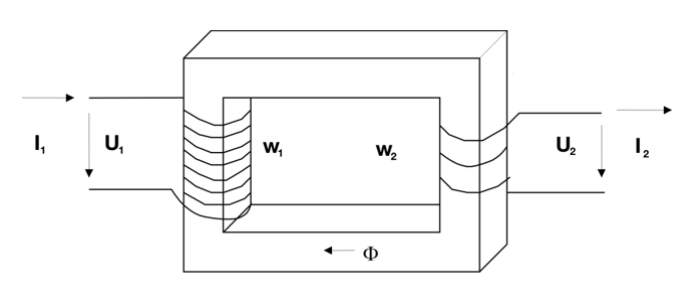
\includegraphics[scale=0.7]{thesis-latex/img/simpletrans.PNG}
    \caption{Composition of a simple transformer}
    \label{fig:simpptrans}
\end{figure}

In a non-ideal transformer primary and secondary winding resistances lead to losses in the windings due to the resistance of the wires. The primary and secondary leakage resistances lead to losses due to the flux leakage out of the transformer core. The core resistance leads to losses due to hysteresis and eddy currents, and the magnetising reactance leads to losses due to the necessary magnetising current to establish the magnetic lux in the transformer core. The copper and iron losses can be represented by ohmic resistors, while the effect of the leakage fluxes are expressed by leakage reactance.

When planning new stations, the expected future utilisation and supply task of the station must be forecasted. Dependent factors are the transformer size and number, as well as the type of supply area, for instance rural or urban. Additionally, the number of cable panels, like MSP cable panels and NSP outlet strips is important to know. Planning of the circuit breaker systems, a connection to remote control technology and the design of the station (if walk-in or compact) are important measures to discuss before installing a transformer. The short circuit strength of the transformer should be defined appropriately to the grid.   


\subsubsection{General Loads}

In LV systems. the loads usually are resistive in nature, with small reactive components due to most buildings being regular households. Hence to model resistive load, a high power factor is needed. For industrial loads, the nature tends to be reactive. 

Household loads in the low voltage networks play a crucial role in the German electricity grid. They are the main source of energy consumption in residential areas and can have a significant impact on the stability and efficiency of the grid. The use of electrical appliances and devices in households, such as refrigerators, washing machines, and lights, can result in large and variable loads on the low voltage network. These loads can cause voltage fluctuations and power quality problems that can affect the performance of other electrical devices in the network.

In addition to their impact on the stability of the grid, household loads also play a role in the integration of renewable energy sources into the grid. With the increasing use of photovoltaic systems and electric vehicles in households, the amount of energy generated and consumed by these sources is increasing. This can result in significant changes in the power flow in the low voltage network and impact the efficiency of the grid. To address these challenges, German utilities are implementing advanced monitoring and control systems to manage the household loads in the low voltage network. These systems use real-time data to optimize the distribution of energy and prevent power quality problems. Additionally, they allow utilities to better integrate renewable energy sources into the grid, making it more efficient and stable.

In conclusion, by understanding their impact and implementing advanced management systems, utilities can ensure the stability and efficiency of the grid while promoting the integration of renewable energy sources in households.



\subsubsection{Cable distribution cabinets}

Cable distribution cabinets (CDC) are most preferably installed at street crossings with severl low voltage cables. The advantages with CDC are the transmission stability due to achieving higher short-circuit power at the node, selective protection, switching options leading to less downtime. The CDC can also act as a "placeholder" for later stations and be an optional grid connection for stand-alone operations. The geographic placement and dimensioning depends on the requirements of the authorities and topology. After commissioning, two reserve outlets should be available to supply temporary connections and charging options.
Existing CDCs must be checked for safety, stability and short-circuit resistance.
It is advisable to provide a switching option after 15-20 grid connections. The number of residential units after which a switching option is necessary depends on the cable utilisation. %planungs
%The Thüga standard is defined as follows: 4, 5, 7 and 10-way cabinet, the short-circuit strength of the CDC must be Idyn ≥ 60 kA, Itherm ≥ 25 kA / 1 s.


\subsubsection{Cables and overhead lines}

In order to connect the loads with the transformers, overhead-lines (OHL) or underground cables are implemented in the grid. An overhead line consists of a transmission tower, insulators, conductors and overhead earth wire. The overhead earth wire protects the tower from direct lightning strikes and must therefore be well grounded in order to discharge the lightning safely. In low voltage systems, overhead-lines are usually connected to low voltage tower neutral conductors. Moreover the towers are usually made out of wood. These towers can only be positioned at a certain maximal distance due to possible sag of the lines in the middle of the tower. The sag depends on the cable tension and weight of the cable. The minimum distance of the overhead line to the ground is defined by VDE 0210-1. %https://www.vde-verlag.de/normen/0200002/din-en-50341-1-vde-0210-1-2013-11.html
Moreover overhead-lines must be able to sustain additional weight, such as ice and snow during winter. The average span for low voltage grids is between 40~m and 80~m. 
OHL are popular due to their low cost and self-healing insulating material, which is air. The airflow's good cooling characteristics lead to non-resticted dimensions by thermal limits. However, OHL disrupt the landscape and need long authorization processes. In densely populated areas and grids with high load density, OHL are often not authorised or technically appropriate. Nowadays OHL are rarely installed in distribution networks. %pt lecture

The operation resistance per unit length of an OHL, $R'$, can be defined by equation \ref{eq:resistohl}, where $R'_{20}$ is the inverse of the cross section times the material constant, $\kappa_{20}$, refering to the specific thermal conductivity of a material at 20°. The thermal resistance, $R'_{\theta}$, depends on the temperature coefficient $\alpha$ and temperature $\theta$. 

\begin{equation}
    R'_{\theta}=R'_{20}[1+\alpha(\theta-20)]
    \label{eq:resistohl}
\end{equation}

On the other hand, cables are mainly placed underground. They have a high operational reliability and are cost-effective for short distances. Thus, underground cables are primarily used in distribution grids. The high capacitance of the cables limit the cable length. Therefore long cables need large and expensive compensation devices. Moreoever cables emit no electromagnetic waves due to the shielding and have higher aesthetic acceptance since they are not visible. However, fault diagnostic and fault clearance is more problematic for underground cables than OHL.  %pt lecture
Especially used at low voltage level is the belted cable. This cable has a non-radial field due to its additional belt insulation between the outer sheath and the conductors. Materials used for cable insulation range from paper impregnated with oil to thermoplastics such as polyethylene (PE).  The operation resistance of cables is calculated similar to OHL in equation \ref{eq:resistohl}. Long distance cables have high impedance which lead to smaller critical clearance time in case of faults. The stiffer the line the longer the critical clearance time. %active distribution

For regular trunk cables copper is the most common material. In some individual cases, the material might vary. Often aluminium is applied if copper cables are financially to expensive. The most common cable diameter for trunk cables in low voltage networks is 150-240 $mm^2$. A greater diameter might be necessary if it is economically important in order to cover future capacity and load increase. %planungs

\subsection{Challenges in the distribution network}
%citaaaation
The German distribution grid faces a number of challenges, including the integration of heat pumps and electric vehicles (EVs) into the energy system. These challenges require the distribution grid to adapt to changing energy demand patterns, while maintaining stability and reliability.

Heat pumps, which use electricity to transfer heat from the ground or air to buildings, are becoming increasingly popular in Germany for heating and cooling. However, their widespread adoption can result in increased energy demand on the distribution grid, particularly during peak hours. This can cause voltage fluctuations and power quality issues, which can affect the performance of other electrical devices in the network.

Similarly, the increasing use of EVs in Germany is also creating challenges for the distribution grid. The charging of EVs can result in large and variable loads on the network, causing power quality problems and requiring the distribution grid to be able to manage the increased energy demand. Additionally, the charging of EVs may result in increased energy demand during peak hours, further exacerbating the challenges facing the distribution grid. To address these challenges, the German Federal Network Agency is promoting the use of smart grid technology and advanced monitoring and control systems in the distribution grid. These systems can help to manage the integration of heat pumps and EVs into the energy system, ensuring that the distribution grid remains stable and reliable.

In conclusion, the integration of heat pumps and EVs into the German energy system presents significant challenges for the distribution grid. However, with the use of advanced technologies and management systems, the distribution grid can adapt to these changes, ensuring a stable and reliable energy supply for customers.

% References:

%     Bundesnetzagentur (2020). Smart Grid: Intelligente Netze für eine Zukunft mit erneuerbaren Energien. [Online]. Available at: https://www.bundesnetzagentur.de/SharedDocs/Publikationen/DE/Themen/Energie/SmartGrids/smart_grid.html [Accessed on: January 30, 2023].

%     European Heat Pump Association (2021). Heat Pumps in Europe: State-of-the-Art. [Online]. Available at: https://www.ehpa.org/wp-content/uploads/2021/06/EHPA-Report-2021-Heat-Pumps-in-Europe-State-of-the-Art.pdf [Accessed on: January 30, 2023].

%     European Commission (2021). Clean Energy for Transport: Electromobility. [Online]. Available at: https://ec.europa.eu/energy/topics/energy-efficiency/sectoral-energy-efficiency/transport/clean-energy-transport-electromobility_en [Accessed on: January 30, 2023].

\section{Grid Analysis}

Grid analysis is a key point in network planning. It serves to determine the maintenance and expansion measures that are necessary in the short, medium and long term, taking into account the existing assets with the aim of guaranteeing technical security, reliability of supply, maximisation of company profits and compliance with the technical framework. 

\subsection{Load Flow}

Whenever evaluating the operation or planning of power systems, a load flow calculation has to assess several factors that might lead to weaknesses in the grid. The power system is analysed under steady-state non-faulted conditions when the system is under maximum demand. This method focuses mainly on the voltage quality, loading of the equipment and optimal flow in the power system. A load flow calculation will determine the active and reactive power flows for all branches, and the voltage magnitude and phase for all nodes. Usually, the network nodes are represented by specifying two out of four of these quantities. Nodes can then be classified as PV, PQ or Slack nodes. For PV nodes, the active power and voltage magnitude are specified. They usually represent generators and synchronous condensers whose active power and voltage magnitude are controlled. Reactive power limits for the corresponding network components are also used as input information under abnormal conditions. PQ nodes specify the active and reactive power, and are usually applied to represent loads and machines with fixed nominal values. As a function of the voltage of the node to which the load itself is connected, the loads might also vary. elements specified as PQ always keep the P and Q within their limits. Lastly, the slack node has a known fixed voltage magnitude and angle. Conventionally, these nodes are also named reference nodes, since the slack node carries out the balancing of the power in the system, through a synchronous generator or an external grid. 

In the AC load flow method, the nodal equations used to represent the analysed networks are implemented using two different Newton-Raphson formulations: Current and Power equations. For distribution systems, especially unbalanced systems, the current equations converge better. %equation?

Normal and abnormal conditions? 

A grid can be defined as unbalanced if voltage unbalances occur. These are associated to variations in voltages and currents for three-phase systems when the RMS voltage values or the phase angles become not equal between the three phases. In low voltage systems, voltage unbalances can occur when there is a load imbalance due to an uneven distribution of single phase loads over three-phase power systems. They can also occur due to a large single-phase loading such as when one of the fuses become not operational for three-phase motors. Voltage unbalances can generate overheating within the windings of induction and synchronous machines. %https://www.sciencedirect.com/science/article/pii/B9780128498699000041 kopiert
For unbalanced systems, under normal operating conditions, during each period of one week, 95\% of the 10 min mean r.m.s. values of the negative phase sequence component (fundamental) of the supply voltage shall be within the range 0\% to 2\% of the positive phase sequence component (fundamental). %https://ieeexplore.ieee.org/stamp/stamp.jsp?tp=&arnumber=7161058 gucken ob es stimmt

Voltage quality is one of the quantities observed during a load flow calculation. It describes the stability of the physical magnitudes of the voltage in relation to nominal values, for instance the effective value or frequency. In other words, voltage stability refers to the ability of a power system to recover from a disturbance and return to a steady-state voltage operating condition that is within upper and lower bound operating thresholds. Norm DIN EN 50160:2011-02 states that under normal operating condition, by exclusion of voltage interruptions, in each period of one week 95\% of 10-minute mean RMS value of power supply voltage within the range of Un of ±10\%, where Un is the nominal voltage of the system. Hence, the network operator has the responsibility to ensure a voltage between 90\% and 110\% of the nominal value. Moreover, all 10 min RMS values of the supply voltage shall be within the range of Un + 10\%/-15\%. Norm VDE-AR-N4105 states, independent of the previous norm, that the distributed generation systems have a requirement to keep the voltage at any node in a range of 97\% to 103\% of the nominal value. %state the norm here

The load flow method will also calculate the loading of the components of the grid. The loading limit depends on the (n-1) criteria, which defines that after the failure of a network resource, it is possible to supply all connection users again after a reasonable time. This can be via a network switchover or short-term use of emergency power systems. In low voltage grids, a (n-1) criteria is not obligatory. However, it can improve the life time and safety of the grid components. For transformer station, a thermal heating above rated temperature limit can be avoided by setting the permanent loading limit at 55-70\%. In case of grid failure, a temporary limit is allowed of 130\% for transformers with oil isolation and 110\% for cast resin isolation. For cables the permanent loading limit is at 50-60\%, with a temporary loading limit of 100\% for PE cables and 120\% for VPE and paper cables. For cables, the maximums are depending on the type of isolation. These values can be found in norm DIN VDE 0276. %reference to norm und planungsgrundsätze thüga


\subsection{Short-Circuit}

Although short-circuits usually are uncommon, power systems must be designed adequately for loads to be reliable in a short-circuit event. A short-circuit condition generally causes large uncontrollable current flows, which if not properly detected and handled can result in equipment damage, the interruption of large areas, as well as placing personnel at risk. Short-circuit happens when an accidental or intentional conductive path between two or more conductive parts force the electric potential differences between these conductive parts to be equal or close to zero. In this case an over-current results, named short circuit current (SCC). Causes for short-circuit can happen due to lightning discharge in exposed equipment, for instance overhead lines, premature ageing of the insulation due to overloading or heating, atmospheric or industrial salt growth, equipment failure or inappropriate system operation.  
 
 To check ratings of network equipment during the planning stage, short-circuit calculations are interested in obtaining the maximum expected currents to dimension equipment properly and minimum expected currents to aid the design of the protection scheme. In Europe, the most common and accepted standard for AC systems in planning environments is the IEC 60909/VDE 0102 method. However, for system operation environments, where the exact network operating conditions are known, the accuracy of this approximated method is insufficient. In that case, the superposition method is necessary. 
 
The IEC 60909/VDE 0102 method does not require system loading information. Alternatively, a specific safety factor, c-factor, regulates the nominal voltage at the point of fault in order to produce high or low results depending on the user specific requirements. Before calculating the short-circuit event, a single or multiple faults are being simulated by introducing an equivalent voltage source at the fault location. The R/X ratio, machine characteristics, synchronous generator type of excitation system, contact parting time, type of network and fault location are the necessary physical quantities to calculate the initial symmetrical short circuit current. An initial fictitious symmetrical short-circuit power, $S_k^{''}$, is determined by the product of the initial symmetrical short-circuit current, $I_k^{''}$, and the nominal system voltage, $U_n$, shown in equation \ref{eq:initialscc}.

\begin{equation}
    S_k^{''} = \sqrt{3} U_n I_k^{''}
    \label{eq:initialscc}
\end{equation}

For meshed networks, three types of calculation methods exist. The first method is called \textbf{Uniform Ratio R/X} where the $\kappa$ factor is determined based on the smallest R(X of all the branches contributing to the short-circuit current. The second method is the \textbf{Ratio R/X at the Short-circuit Location}, where the $\kappa$ factor is multiplied by 1.5 to cover inaccuracies by using the ratio R/X from a network reduction with complex impedances. At last, the \textbf{Equivalent Frequency}, calculates an equivalent impedance $Z_c$ from the short-circuit location by assuming a frequency, $f_c$, equal to 20~Hz. The R/X ratio is then defined by equation \ref{eq:R/X}. For meshed networks, the last method is the most appropriate.  

\begin{equation}
    \frac{R}{X} = \frac{R_c}{X_c} \frac{f_c}{f}
    \label{eq:R/X}
\end{equation}

$R_c$ and $X_c$ are the real and imaginary part of the equivalent impedance respectively. $R$ and $X$ are the equivalent values at nominal frequency, $f$, with 50~Hz. Eventually the $\kappa$ factor is defined by equation \ref{eq:kappa}, which in turn gives the peak short-circuit current, $i_p$, defined in equation \ref{eq:peakscc}.

\begin{equation}
    \kappa = 1.02 + 0.98e^{-3R/X}
    \label{eq:kappa}
\end{equation}

\begin{equation}
    i_p = \kappa\sqrt{2}I_k^{''}
    \label{eq:peakscc}
\end{equation}

%symmetrical sc breaking current
In the most common situation, the fault occurs far from the generator. In the LV case the response is represented by a reactor-resistance circuit and the short circuit currents do not have damped alternating components. The initial, $I_k^{''}$, steady state, $I_k$, and breaking $I_b$, short circuit currents are equal and the positive and negative sequence impedances are equal. The peak current is then calculated in the same manner as \ref{eq:peakscc}. In the case when the fault occurs close to the generator, the emf force is assumed constant and the internal reactance of the machine is variable. Three stages of reactance develop, illustrated in figure \ref{fig:reactanceneargenerator}. The first 10 to 20 ms show the subtransient state, followed by the transient state up to 500ms and eventually reach the steady-state. The breaking current defines the breaking capacity of the time delayed circuit breakers and is only required when the fault is near the generator. The breaking current is calculated by the factor $\mu$ in equation \ref{eq:breakingcurrent}.

\begin{equation}
    I_b = \mu I_k^{''}
    \label{eq:breakingcurrent}
\end{equation}

The factor $\mu$ depends on the minimum time delay $t_{min}$ and the ratio between the initial and rated generator current. The values can be found in the IEC 60909 norm. 

\begin{figure}[ht]
    \centering
    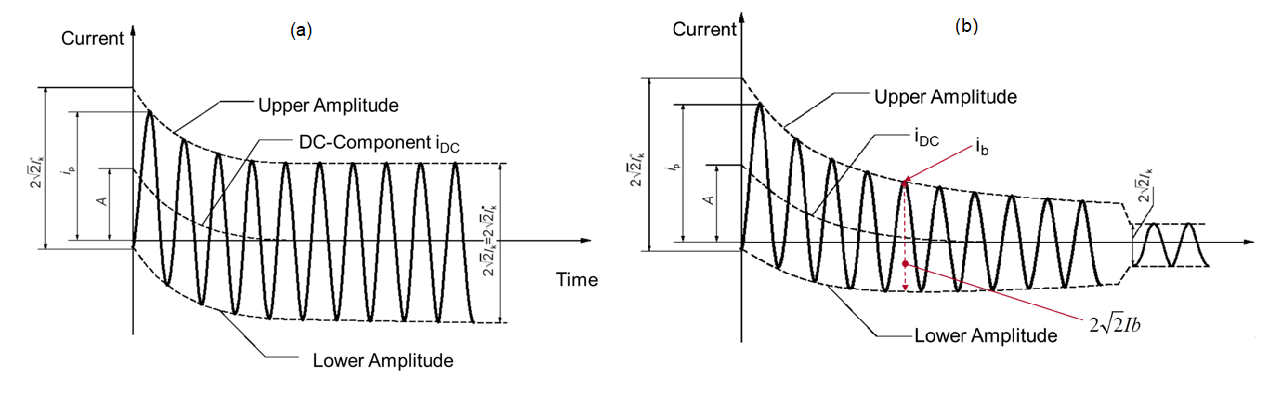
\includegraphics[scale=0.4]{thesis-latex/img/FarGenSC.PNG}
    \caption{Evolution of the short-circuit current over time when (a) far or (b) close to the generator %IEC60909
    }
    \label{fig:reactanceneargenerator}
\end{figure}

%steady state sc current
% In meshed networks, the maximal steady state short-circuit current, $I_{k,max}$, is equal to the initial current and the minimum, $I_{k,min}$, is equal to the minimal initial current. 

On the other hand, the complete method produces results by superposition when given a realistic pre-fault loading of the system. In the faulted state, all voltage sources are shorted whilst an additional voltage source is connected at the fault location injecting a voltage equal opposite to the pre-fault voltage at that location, determined from the load flow calculation. %hier mehr schreiben??

Short circuit can be phase-to-earth (80\% faults), phase-to-phase (15\% of faults), three-phase (only 5\% faults). 

%IEC norm und UserManual Power Factory

% \subsection{Harmonic voltage and THD}
% Under normal operating conditions, during each period of
% one week, 95 \% of the 10 min mean r.m.s. values of each
% individual harmonic voltage shall be less than or equal to the
% values given in [1] when the limit value for the 15th voltage
% harmonic is 0.5\% of nominal voltage. Moreover, the THD of
% the supply voltage (including all harmonics up to the order 40)
% shall be less than or equal to 8 \%. %https://ieeexplore.ieee.org/stamp/stamp.jsp?tp=&arnumber=7161058

%\subsection{Flicker}

\subsection{Quasi-Dynamic simulation}
%simultaneity factor

Due to the complexity of the network, it may be difficult to intuitively understand which operating cases and network states lead to faulty conditions. To identify the most unfavourable operating conditions, often several different load flow simulations with different operating conditions must be carried out. In addition, most operating parameters have an underlying time dependence, hence the grid model also has a temporal dependence. A load is time dependent due to daily and seasonal cyclic load variations. Renewable energy sources such as solar power generation and wind power generation vary with solar radiation and wind speed. Grid variants, maintenance shutdowns, faults and unforeseen outages usually have a certain time dependency. Finally, device performance may also change due to wind and temperature influences. By analysing chronological load flows, the time interval in seconds is not important, but more of minutes to hours or month to years, depending on the operation case. Voltage stability, for instance, needs an approximate interval of 10 minutes. Therefore a quasi-dynamic simulation can be a practical tool in those situations. 

A quasi-dynamic simulation is a combination of steady state load flow analysis with during a certain time interval with a defined time-step. This tool is particularly suitable for planning studies in which long-term load and generation profiles are defined and the grid expansion is modelled with the help of variants and expansion stages. Especially for load flow and the irregular energy production of renewable energies, the quasi-dynamic simulation is a great method in order to spot the most critical time slots or season during grid operation.  

\subsection{Simultaneity factor}

In quasi-dynamic simulations and load flow calculations, the simultaneity factor of generation and load units must also be defined. The simultaneity factor or coincidence factor is used to estimate how heavily a supply system will typically be used in order to dimension it appropriately. If, for example, the supply lines for water, electricity, gas and communication are designed for a new development area, on one hand the supply must be ensured at peak times while on the other hand there should be no oversizing due to higher investment costs. If all connections are used at 100\% at the same time, then the value of the factor is 1. If only 10\% of the power is used, the simultaneity factor is accordingly equal to 0.1.

However, the simultaneity factor itself is not relevant for the network operations, but the resulting power contribution, which results from the multiplication of the simultaneity factor with the number of charging points and the charging power. Even if the simultaneity factor often decreases with increase of loads, the absolute power contribution increases continuously. In addition, when dimensioning the network, the time correlation of the new load contribution with the other original loads must be taken into account.

\section{Heat Pumps}

A heat pump (HP) is a device that uses technical work to absorb thermal energy from a lower-temperature reservoir and transfers it with help of the electrical drive energy as useful heat to a higher-temperature system to be heated. The process is described in Fig. \ref{fig:hpschema}. The low-temperature reservoir is connected to a heat exchanger, the evaporator, being the connection between the energy source, for instance outside air, and the refrigerant. As low pressure liquid, the refrigerant has a lower boiling point than the energy source. %whats a usual refrigerant
Hence the outside air evaporates the refrigerant by passing by the evaporator. The latent heat is being absorbed at the boiling point. In the next step, as low pressure gas, the refrigerant enters the compressor. During the compression the refrigerant transforms into a hot high pressure gas and enters the second heat exchanger, the condenser. Due to its pressure, the boiling point temperature is higher in the condenser than in the evaporator. On the other hand the heating fluid, entering the heating system of the house, has a lower boiling point than the refrigerant. Hence the refrigerant condenses to a liquid and releases its latent heat to the heating fluid. After leaving the condenser, the refrigerant leaves the condenser as warm liquid and passes through the expansion valve in order to reduce the pressure and vaporise.~\cite{DINCER2015131}

\begin{figure}[ht]
    \centering
    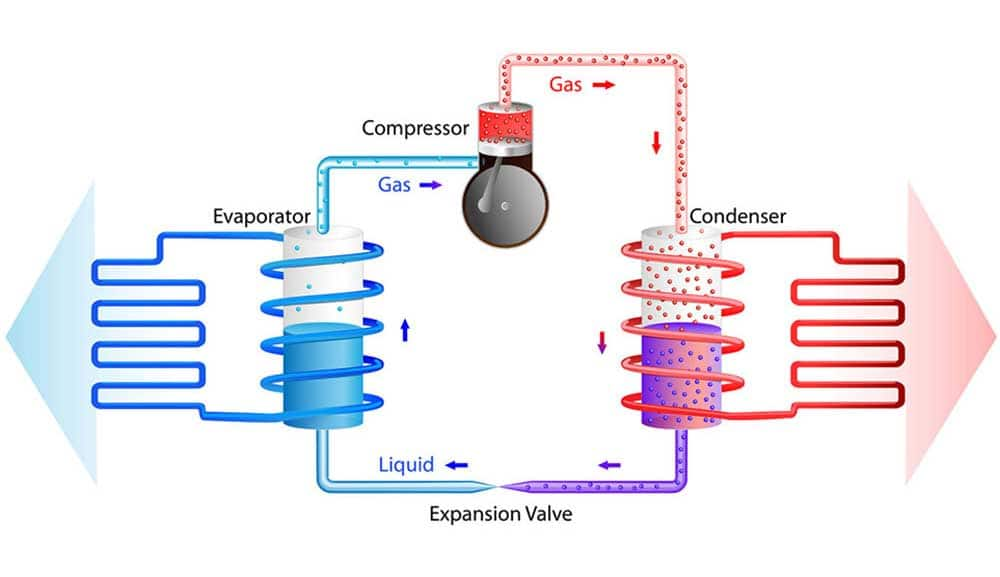
\includegraphics[scale=0.3]{thesis-latex/img/hpschema.jpg}
    \caption{Schematic representation of the working principle of a heat pump \cite{}.%https://sauermanngroup.com/en-US/insights/heat-pumps-how-do-they-work-and-how-maintain-them
    }
    \label{fig:hpschema}
\end{figure}

The lower-temperature reservoir can have different sources. The most commonly used reservoirs are the ambient outside air, geothermal probes installed in the ground, or the groundwater. Another source is waste water. Depending on the technology, technical characteristics, for instance, efficiency or operation hours, vary. Every electrical heat pump (EHP) has an additional auxiliary heat pump (AHP), also known as a heating rod, which operates on the coldest day of the year. The EHP by itself should be able to cover 80\% of the peak thermal load on the coldest days of the year~\cite{navarro-espinosa_probabilistic_2014}. Studies state that a sizing of 80\% gives close to optimum $CO_2$ and running cost savings, while a 60\% sizing covers the major amount of heating requirement~\cite{navarro-espinosa_probabilistic_2014}. Hence the sizing should lie between these two limits in order to restrict capital cost and installation area. For the AHP, it should have an annual load ratio of not more than 3\% in order to stay in the previously stated margin. %https://www.ise.fraunhofer.de/content/dam/ise/de/downloads/pdf/Forschungsprojekte/BMWi-03ET1272A-WPsmart_im_Bestand-Schlussbericht.pdf
Additionally the AHP supports the EHP regarding frost protection and emergency operation if the heat pump fails. Usually, heating rods have a power between 2.5~kW to 10~kW.%https://www.ise.fraunhofer.de/content/dam/ise/de/downloads/pdf/Forschungsprojekte/BMWi-03ET1272A-WPsmart_im_Bestand-Schlussbericht.pdf


A heat pump's efficiency is defined by the seasonal performance factor (SPF), which is defined by dividing the energy of the output thermal heat, $Q_{th}$ by the energy of the input electricity, $W_{el}$~\cite{DINCER2015131}. In other words, the SPF is the average coefficient of performance (COP) of a heat pump over the full heating season. The COP is the SPF but only at one specific time. The COP is highest during summer and coldest during winter since the outside temperature is proportional with the COP. The COP can vary between 1.5 and 6.0~\cite{SARBU2017347}. 

HPs are in general more costly to install than other heating systems such as furnaces or electrical heaters. Over long-time use, however, the HP can prove to be cheaper. If powered by renewable energies, the HP can also be a sustainable heating source.  

Air source heat pumps (ASHP) use a ventilator to absorb the ambient outside air as the lower-temperature reservoir. ASHP are easy and simple to install as they do not require any additional constructions. The ventilator unit will be visible outside of the property, similar to an air-conditioner. Hence, the fans might generate noise during operation. In general, the noise is tolerable and increases only on the coldest days. The SPF reaches 3.3 in residential buildings and can reach 4.6 if integrated within a smart grid. 
%file:///C:/Users/THVMERSA/Th%C3%BCga%20Aktiengesellschaft/FB_EN%20-%2003_EN-S/Organisation/08_Werkstudent,%20Entsendungen%20und%20Studienarbeiten/Merzoug/Masterarbeit/W%C3%A4rmepumpen/A-EW_273_Waermepumpen_WEB.
The ASHP is the only heat pump suitable for old period buildings. %https://www.bosch-thermotechnology.com/de/de/wohngebaeude/wissen/heizungsratgeber/waermepumpe/waermepumpen-vergleich/

Ground source heat pumps are using geothermal probes installed as a ground loop in an outdoor space, usually the garden. The GSHP is more complex and expensive to install due to the necessity of the installation of the geothermal probes. However the unit is not visible on the outside and the garden can be used in its full functionality. Moreover, the SPF reaches 4.3 in residential buildings and can reach at value of 4.7 in a smart grid integration. %file:///C:/Users/THVMERSA/Th%C3%BCga%20Aktiengesellschaft/FB_EN%20-%2003_EN-S/Organisation/08_Werkstudent,%20Entsendungen%20und%20Studienarbeiten/Merzoug/Masterarbeit/W%C3%A4rmepumpen/A-EW_273_Waermepumpen_WEB.pdf
The AHP is less used for the GSHP compared with the ASHP. Due to high heat capacity of water compared to air, the efficiency rate is more stable than for ASHP. %https://www.bosch-thermotechnology.com/de/de/wohngebaeude/wissen/heizungsratgeber/waermepumpe/waermepumpen-vergleich/

Groundwater heat pumps (GWHP) removes the groundwater from a well and delivers it to the HP with help of a pump. This lower temperature reservoir serve then as the energy source of the HP. Due to the constant groundwater temperature over the seasons, the power input of the GWHP varies even less for the HPs above. %https://www.bosch-thermotechnology.com/de/de/wohngebaeude/wissen/heizungsratgeber/waermepumpe/waermepumpen-vergleich/
Hence, this technology can reach an SPF of 5.0 in residential buildings. %https://www.researchgate.net/publication/350473990_On_the_real_performance_of_groundwater_heat_pumps_Experimental_evidence_from_a_residential_district 

The performance of heat pumps also depends on the building's energy efficiency. The European Union has established energy efficiency standards in order to be able to separate buildings in different categories, displayed in Table \ref{tab:kfw}.

\begin{table}[!ht]
    \centering
    \caption{European energy standard}
    \begin{tabular}{c|c}
        \textbf{Heating demand} & \textbf{Energy standard} \\
        \textbf{kWh/m$^2$} & \\
        \hline\hline
        $\leq$ 25 & A \\ 
        $\leq$ 50 & B \\ 
        $\leq$ 100 & C \\ 
        $\leq$ 150 & D \\ 
        $\leq$ 200 & E \\ 
        $\leq$ 250 & F \\ 
        $>$ 250 & G \\ \hline
    \end{tabular}
    \label{tab:kfw}
\end{table}

Accordingly to this table, a building with an energy standard of 90 kWh/m$^2$ will have the energy standard C. In Germany, over the years the regulations of energy standard for building became stricter. Buildings built before 1980 had a minimum requirement of 300 kWh/m$^2$, while the requirement in 1995 was 100~kWh/m$^2$~\cite{Bundesregierung_1994}. With improving energy efficiency in buildings, the heat pumps are more effective, has smaller dimensions and becomes financially more attractive. 


%COP equation

\section{Battery Electric Vehicles}

An electric vehicle is a car which is partly or fully driven by using electricity. For instance a Plug-In electric vehicle mainly uses a conventional combustion engine but has an optional internal rechargeable battery pack, which can provide electricity to its electric machine. On the other hand a battery electric vehicle (BEV) exclusively uses chemical energy stored in rechargeable battery packs, with no secondary source of propulsion. The advantage with this type of car is its zero emission drive and can be charged at home. The amount of battery electric vehicles on German streets increases continuously. Therefore, it is important to identify the impact of the BEV on the public electricity grid. 

\subsection{Battery technology of electric vehicles}

BEV generally have lithium-ion batteries installed. The battery size and capacity varies depending on the car and can consequently only tolerate a certain amount of charging power. On average BEV used in rural areas have a consumption of 28~kWh/100~km, while urban areas have an average consumption of 42~kWh/100~km~\cite{VDEFNN_2021}. 

If this limit is exceeded, the function of the battery can be severely impaired. Several studies state an increased ageing rate at long charging periods at temperatures above 40°C~\cite{yang_asymmetric_2019}. Moreover, the high charging current in fast charging increases the risk of individual cells being damaged by overpotential~\cite{yang_asymmetric_2019}. Hence the greater the battery capacity, the more power the battery can be charged with. 


\subsection{Charging of battery electric vehicles}

Unlike other types of customers, the consumption profiles of charging points for electric vehicles have greater uncertainties, since these profiles, especially the mobility behaviour, depend on the individual vehicle user. Network operators can't foresee load behaviour regarding operating experience. Nonetheless, they need to assume charging behaviours to identify specific load behaviour in order to expand the grid in an optimal and future-oriented way.  

Studies show that the most frequent charging pattern is morning and afternoon. 50\% to 80\% of charging events occur at home~\cite{lee_exploring_2020}. Workplace and commute charging is the next more favourable option, especially if it is for free. 15\% to 20\% of charging events occur at workplaces~\cite{lee_exploring_2020}. Only 5\% of charging events occur at publicly accessible charging locations, for instance shopping malls and parking lots~\cite{lee_exploring_2020}. At house and workplaces, the charging power stays mostly below 11~kW, while public accessible chargers might vary between 3.7~kW and 150~kW. 

The distribution of the charging start time can be extracted by analysing the probability of arrival when assuming that the charging process happens after arrival. In the work week, the arrival time is expected in the morning hours is the highest at the workplace, while the arrival at the place of residence is concentrated in the late afternoon and early evening hours. The driving behaviour from Mondays to Fridays is represented in Fig. \ref{fig:drivingpattern}. Due to the irregular daily routines on weekends, the arrival times are not especially concentrated and occur in a relatively even way. 

\begin{figure}[ht]
    \centering
    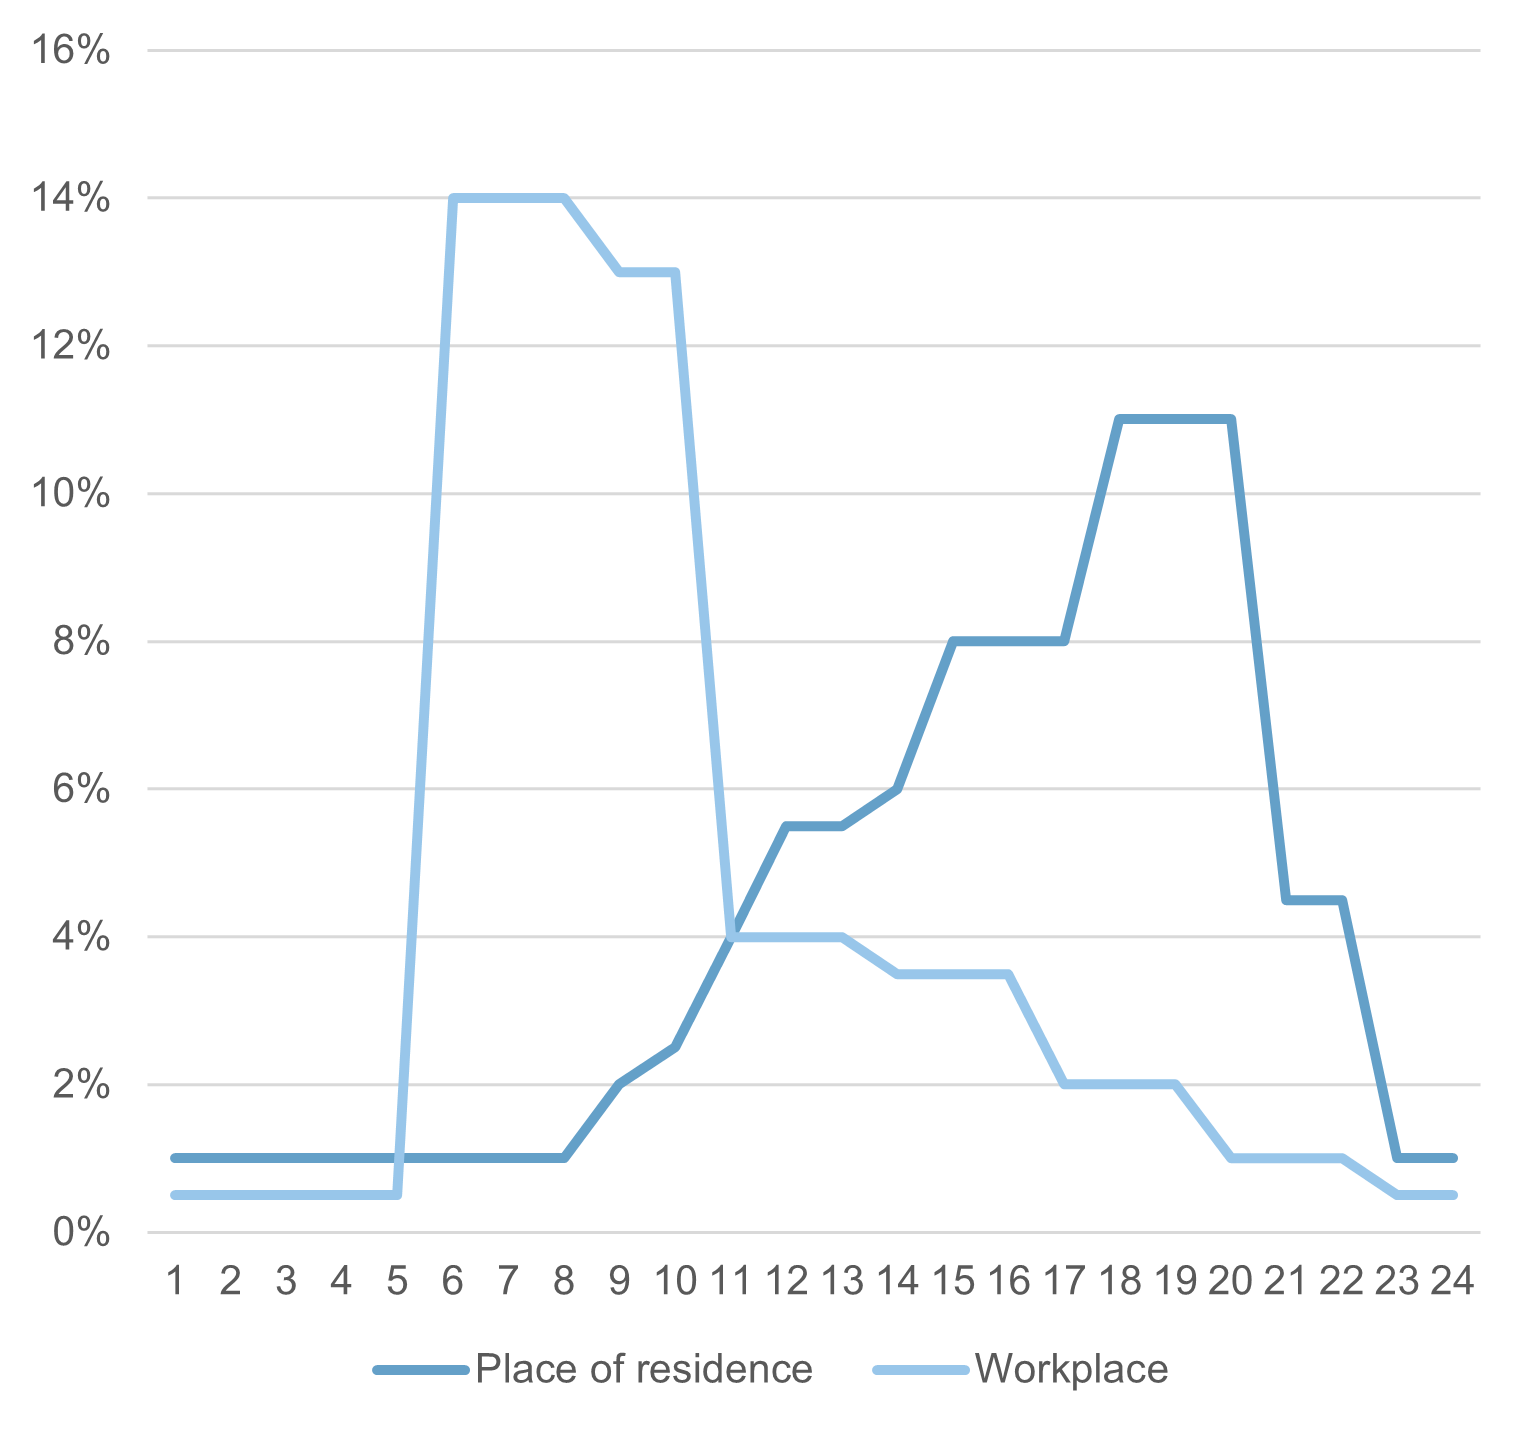
\includegraphics[scale=0.8]{thesis-latex/img/charging probability.png}
    \caption{Hourly probability of arrival depending on place of residence and workplace~\cite{VDEFNN_2021}}
    \label{fig:drivingpattern}
\end{figure}

Depending on the area, the daily driving range varies. For urban BEV, the average daily range lies at 31~km, while the rural areas have a range of 42~km~\cite{VDEFNN_2021}.




\section{Grid reinforcements}
%mona und nova prinzip - julia bei teams
In order to adapt the network infrastructure to the new requirements, it can not only be expanded, but also optimised or strengthened. Hence, the existing distribution capacities can be increased or used more efficiently. The optimum between the expansion of grid capacities due to high load and the temporary limitation of the maximum feed-in of renewable energies must be examined as well. These characteristics are important to consider in order to replace or optimise the existing components in the grid. The most common grid reinforcement options will be described underneath of this section. 

Elements applied in grid reinforcement can be split up into three categories: grid-optimising equipment, grid-optimising operations and grid-oriented measures. The two first categories only differ in their nature of cost. The optimising resource category is shaped by the investment costs of the elements, CAPEX, while the optimising operation category is defined by its elements operational cost, OPEX. The third category does not contain any physical elements, but the management and regulation of elements impacting the grid. 

\subsection{Grid-optimising equipment}

Grid-optimising equipment contain elements that often already exist in the current grid and can be strengthened or must be replace. This category can also be seen as a conventional way of improving the distribution grid and has been the most commonly used grid reinforcement method. 

%\subsubsection{Transformer replacement}
%RONT or change transformer
%always state the cost 

In the case of transformer replacements, an existing local network transformer (ONT) is replaced by a higher rating transformer, usually with a rated apparent power of 400~kVA or 600~kVA. Mostly, these transformers operate at better efficiencies and deploy more advanced technologies~\cite{noauthor_dena_nodate}. 

%\subsubsection{Cable and overhead line expansion}
%parallel or new
%impedance of cables
%https://www.allaboutcircuits.com/textbook/alternating-current/chpt-14/characteristic-impedance/

Another grid-optimising resource is the expansion of cables or overhead lines. Mainly, there are two methods to consider for improving cables reliability. First, the old cables are totally replaced by new cables with higher load flow capabilities, which will allow the new cables to handle higher load flows with no concerns. The other option is to add a parallel line along the old one that usually has the same capacity which work as splitting the load flow equally between the two parallel lines allowing the cables to handle the increasing load flows. The main concept for these two solutions is to decrease the impedance of the lines. A standard cable applied as parallel cable for grid optimisation is the NAYY 4x120 or 4x150.~\cite{amprion_underground_2017,mona}

Usually the standard ONT replacement and cable and OHL expansion are classified as the conventional grid expansion. This category can be combined with nearly any other technology, is scalable and already established~\cite{monamaßnahmen}. However, due to the visual pollution and necessary construction work, conventional grid expansion has a great impact on flora and fauna, and hence also the regional acceptance is rather low. Moreover the investment costs are high to be accepted by regulation, but the operational costs are relatively small and no additional ICT is necessary.

Contrary to the standard ONT, a regulated local network transformer (rONT) can be installed. In that case, the current transformer is replaced with a rONT with the same size and rating. The rONT, though, is equipped with an on-load tap-changer that can dynamically adjust the set-point depending on the passing power. One type is the so-called Voltage Regulated Distribution Transformers (VRDT) perform in a different way than conventional transformers by adapting to voltage variations in MV/LV grids with no interruptions to the operation. Which provides an economical and compact asset to the network. The on-load tap transformer is specially equipped with voltage changing capabilities by adjusting the tap position for real-time grid adjustment. This results in changing the voltage level of the nodes within the grid, such that it keeps the operation within the acceptable limits. The allowed tap positions are determined at the design stages, and in operation the transformer can alternate freely between these positions. Nonetheless, it is limited around a reference point which is usually specified as the standard operation point of the grid.~\cite{9543749,sojer_voltage_2017}

The line voltage regulator can be used in both medium and low voltage. It only acts on the subordinate network section and can be used if the voltage change is to high.  The use of a low-voltage linear regulator can be useful in a single circuit with a conspicuous load-voltage ratio, e.g. settler farms with an impedance-related voltage increase or decrease, as well as in the case of a supply to transmission masts. The location of the LVR should be close to the relevant customer installation. If necessary, upstream network areas can also be optimised. The single-phase control can offer advantages especially for individual, asymmetrical customer behaviour. 

rONT and LVR are mainly used in areas with voltage issues and without thermal issues. By implementing these technologies in the grid, the installed capacity of renewable energies can be increased simultaneously. The regional acceptance is high. Theses technologies have small impacts on the operational cost but additional ICT is not necessary.~\cite{monamaßnahmen}

\subsection{Grid-optimising operations}

The most common element in grid-optimising operations is the reactive power control. In this situation, the reactive power of units connected to the grid can be controlled and regulated. Typical components are PV-panels, electric vehicles, home storage systems or speed controlled heat pumps. All these components are originally DC units which must be transferred to AC in order to be able to connect to the grid. Hence inverters, transforming DC voltage to AC voltage create reactive power. The available reactive power depends on the apparent power of the installed components. In reactive power control, inverters can curtail the active power or consume the reactive power to avoid the excessive high voltages. When load is small, system generates reactive-power, that should be absorbed. At the same time at large loads it consumes plenty of reactive energy that needs to be produced. This can be done by changing the firing angle of the thyristors. For example, higher value of firing angle brings out bigger phase shift between the current and voltage which results in larger reactive power demand or vice-versa. In the grid, the deployed reactive power control is similar for every inverter.~\cite{power_transmission,mona}

For reactive power control, the hosting capacity of the grid regarding renewable energies increases due to the fact that a lot of those technologies have access to inverters. The investment costs are relatively low to none. Additionally a targeted reactive power controller can actively support the reactive control in higher grid levels through the inverter in households.~\cite{monamaßnahmen}

Another typical grid-optimising operation is the method of topological switching operations (TSO). This operation denotes the additional meshing of type networks by closing switches in junction boxes. The evaluation of the switching operation is carried out in two networks in order to compare the impact of additional switches. During operation time switches might need to open or close in order to dismantle high loading.~\cite{mona}

TSO has low potential for grid relief and is usually applied for fault occurences. However, TSO has no impact on acceptance or the environment, has low cost and does not demand any additional ICT.~\cite{monamaßnahmen}

\subsection{Grid-oriented measures}

Furthermore, grid-oriented measures can make the individual elements of the grid more flexible, such as increasing load management on the demand side (DSM), the use of storage facilities, the linking of decentralised systems to virtual power plants or the construction of intelligent networks in order to Coordinated control of network components, storage and consumers. These can be used to reduce the need for grid expansion.

Due to the increasing electrification in the heat sector, the reinforcement possibilities of hybrid grids, for instance Power2Heat (P2H), measures in the low-voltage grid are worth examining. These include the flexibility of heat pumps, as well as electric storage heaters. A possible flexibility is able to b attained by considering self-consumption optimisation, where the installed system and ICT infrastructure cooperate to minimise the residual household load. On the other hand, a voltage controlled flexibility of heating units can be an option, where the local voltage measurement serves as a trigger to increase or decrease heat production.~\cite{mona}

Hybrid networks is a proven one and highly scalable technology with great existing potentials. The cooperation between heat and electricity sectors is encouraged by politics and is low in cost regarting flexibility for energy systems.~\cite{monamaßnahmen}

Another promising idea is the storage district concept. In order to support the grid, battery storage units with an output between 50 and 500~kW are installed in specific regions of the grid, usually in the middle of the weakest line. The dimensioning is based on regulation of 60\% of energy generation in the grid area. The ratio between the capacity of the grid to the installed power of the battery has a rate of 3:1. For this option, two different flexibility aspects can be controlled. The first one is the voltage controlled operation, where the charging and discharging controller reacts on the local voltage measurements at the battery storage system. The storage unit would be controlled by the grid operator. The second option, is to optimise the self consumption of the district in order to maximise the share of self-consumption in the area.~\cite{mona}

District concept offers the possibility to increase the degree of self-sufficiency grid area. Due to missing legal definitions in the EnWG uncertainties prevail. The operation might cause additional load. High consumption of resources. Small reaction time leads to very dynamic and flexible operation. BESS helps suppress the surplus of PV, reduce the emission of CO2, increase of market integration and politically supported. self-sufficiency can help.~\cite{monamaßnahmen}

The last flexibility reinforcement is the control of electric vehicles, also known as Vehicle2Grid (V2G). The charging capacity depends on the availability of a
charging station and its nominal power. Here again, voltage-controlled charging reacting to the local voltage measurement or charging control optimised for self-consumption are the possible evaluation options.~\cite{noauthor_peak_2019}


The targeted loading of electric vehicles needs the implementation of not yet existing charging management. It is to be expected that charging control will be implemented on a voluntary basis or based on incentives. There is currently no corresponding one compensation model, nor a clear legal or regulatory regulation. The smart meter rollout offers the infrastructure for control of electric vehicles.~\cite{monamaßnahmen}

%Several flexibility options exist in order to make the grid more flexible when needed. The most common option is peak shaving, which is the process of mitigating high demand peaks. Operators can face economic challenges due to peak demand charges. To even out the peak loads, effective methods such as demand side management (DSM), energy storage system (ESS) or vehicle to grid (V2G) operation are used~\cite{noauthor_peak_2019}. Demand side management aims to balance customers electricity consumption and optimise their energy use. This management can be categorised by the energy efficiency or demand response. By improving the energy efficiency, the same service can be accomplished with less energy drawn from the grid~\cite{uddin_moslem_review_2018}. Battery storage is a technology that enables power system operators and utilities to store energy for later use. A battery energy storage system (BESS) is an electrochemical device that charges (or collects energy) from the grid or a power plant and then discharges that energy at a later time to provide electricity or other grid services when needed. One extension of the energy arbitrage service is reducing renewable energy curtailment. System operators and project developers have an interest in using as much low-cost, emissions-free renewable energy generation as possible~\cite{leish_grid-scale_2019}. Appropriately sized BESS can also provide longer-duration services, such as load-following and ramping services, to ensure supply meets demand~\cite{leish_grid-scale_2019}. V2G operation describes a system in which an electric vehicle communicates with the power grid to either returning electricity to the grid or by throttling their charging rate in order to shave the demand response~\cite{and_ShuangGao}.

%battery storage systems

\chapter{Market situation and future growth}

\section{The German electricity market}
%peak shaving, dsm, 
The electricity market in Germany consists of various sub-markets with individual price signals. Producers and consumers base their planning on these prices. The transmission system operators compensate for unforeseeable deviations from regularities between supply and demand with control reserves. The balancing energy system ensures the cost-optimal use of supply and demand. The electricity market thus rewards work and performance.

Thanks to the Merit Order, the energy produces with the cheapest price has priority to sell before more expensive energy producers. The energy prices for selling often, represent the production cost. Since renewable energies are the cheapest type of generation, they usually have priority~\cite{Bundesnetzagentur}. 

Contrary to other goods, electricity is hard to store. Hence electricity must be delivered to the end-consumer right after being generated. Therefore electricity prices can vary daily, as well as hourly. For instance, if the supply is high and the demand small, the price decreases and vice versa. The drastic price signals are illustrated in Fig. \ref{fig:pricesignals}.

\begin{figure}[ht]
    \centering
    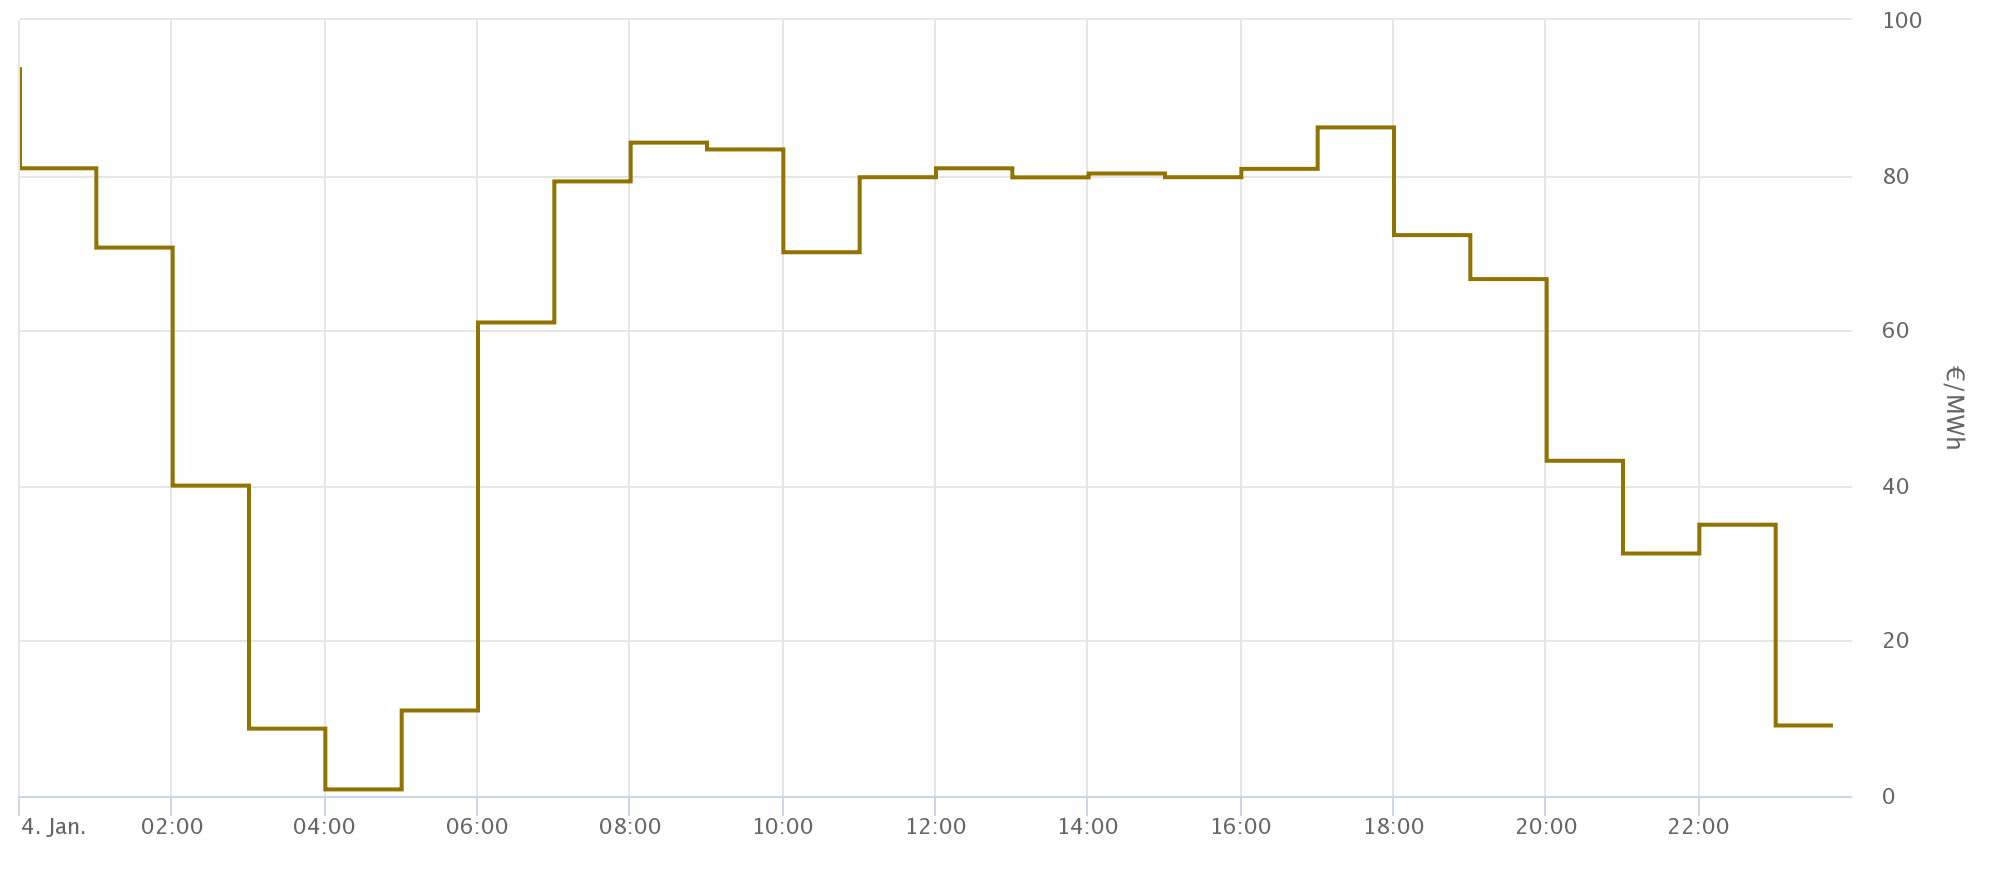
\includegraphics[scale=0.3]{thesis-latex/img/pricesignals.png}
    \caption{Price signals on the German electricity market on the 4th of January 2023~\cite{Bundesnetzagentur}}
    \label{fig:pricesignals}
\end{figure}

Hence the price the end-consumer has to pay eventually depends on the supply and demand ratio at that specific moment. Considering the mentioned graphic, people prefer pulling electricity from the grid when it is cheap, hence at night. However, most people don't need the electricity at that time and have no option to store it. Therefore it is important for the utility grid to have the maximal necessary capacity in a critical case, where all households want to use energy from the grid or feed electricity into the grid. 

%paragraph 14a?
%increasing prices with now dependent and less production (russia)

\section{Future heat pump market}
\label{sec:markethp}

Gas and oil heating are the most commonly used heating structure in Germany by 2019 with 48.2\% and 25.6\% respectively~\cite{BundesministeriumfürWirtschaftundKlimaschutz_2019}. Only a small fraction heats with heat pumps. However, the popularity of heat pumps has increased during the last years due to the Paris Agreement, and moreover so due to the war in Ukraine, leading the gas prices to skyrocket. The most popular heat pump, the ASHP has increased its market share by 33\% in 2021 compared to the previous year~\cite{BWP_2022}.
GSHP has an increase of 12\%~\cite{BWP_2022}. Hence the projection estimates that ASHP will become the most popular heat pump due to its low cost and simple installation, while GSHP will be at the second place, followed by the GWHP on third~\cite{marekmiara}.

Additionally, the federal government is faced with the task of tripling the installation of heat pumps by 2024. The German economy minister has claimed to increase the installation of heat pumps by installing a minimum of 500~000 heat pumps annually from 2024~\cite{tagesschaude_2022}. This will mean 6 million heat pumps by 2030. Moreover the European Union has stated in the Energy performance of buildings directive that by 2030, all residential energy consumption should be renewable in case of technical possibilities~\cite{EPBD_2021}. Subsequently, the heating sector is destined to transition from gas and oil to electric heating.

However, not all households have the technical possibility to install heat pumps, for instance historical buildings or places of worship. Approximately 75\% of all buildings in Germany can use a heat pump as energy source~\cite{agoraWP}. The energy efficiency of buildings is also a limiting factor. Heat pumps can rapidly become financially unattractive in badly isolated buildings due to the high electricity bills. Accordingly, the European Union has decided that all residential buildings must improve their energy standard by standard F by 2030 and by standard E in 2033~\cite{EPBD_2021}.

\section{Future electric vehicle market}

The increase of BEV has been drastic over the last years as well. Especially between 2020 and 2022, the number of BEV has double every year. Including the plug-in hybrid vehicles (PHEV) and the BEV, the ratio is still at 2.2\% compared to the total amount of cars in Germany~\cite{Kraftfahrzeugbundesamt_2022}. Additionally in 2021, 44\% of all newly registered cars had an alternative drive. 

One of the reasons for slow growth might be some inconveniences that still leave potential costumers hesitating. In Germany, 42\% state that the limited driving range is an obstacle to purchase, while 25\% of these costumers would be willing to buy a car if the driving range exceeded 500~km. Even though, an average German citizens spends only 10 days a year exceeding the 400~km range. Another point is the missing public charging access, where 75\% state this fact as an obstacle~\cite{ConsorsFinanz_2019}. Nonetheless, the BEV trend is increasing and might become the leading vehicle technology in later years. %thüga quelle

In order to boost the BEV sales, the German government has set has a goal that the total amount of BEV should reach 15 million by 2030~\cite{FrankSonntag_2021}. In order to increase the attractiveness of electric vehicles, the government has decided to provide additional appeals. Overall, temporary purchase incentives, further funds for the expansion of the charging infrastructure, additional efforts in the public procurement of electric vehicles and tax measures are being introduced~\cite{elektromobilität_2022}.